\section{Transformer Overview}
\begin{frame}{}
    \LARGE Advanced Computer Vision: \textbf{Transformer Overview}
\end{frame}

\begin{frame}{Transformers}

\begin{figure}
\centering
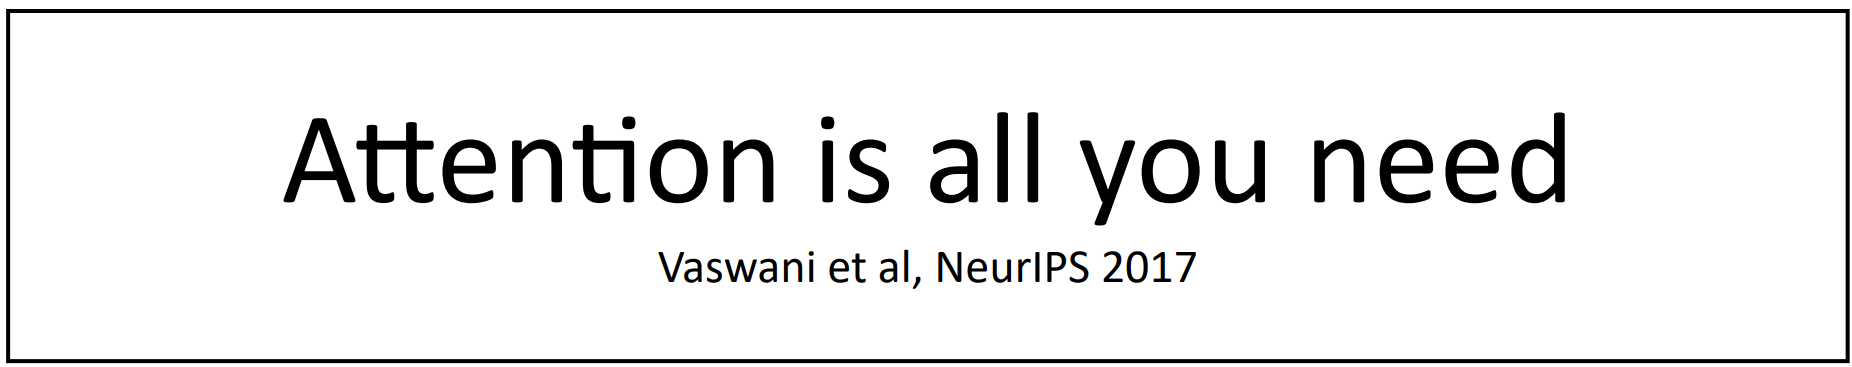
\includegraphics[width=1.0\textwidth,height=1.0\textheight,keepaspectratio]{images/advanced-cv/transformers_1.png}
\end{figure} 
    
\end{frame}

\begin{frame}{Transformer Block}

\begin{columns}
    \begin{column}{0.5\textwidth}
        \begin{itemize}
            \item \textbf{Input:} Set of vectors $\mathbf{x}$
            \item \textbf{Output:} Set of vectors $\mathbf{y}$
            \vspace{0.5cm}
            \item Self-attention is the only interaction between vectors!
            \item Layer normalization and MLP operate independently on each vector.
            \item Highly scalable and highly parallelizable.
        \end{itemize}
    \end{column}
    \begin{column}{0.5\textwidth}
        \begin{figure}
        \centering
        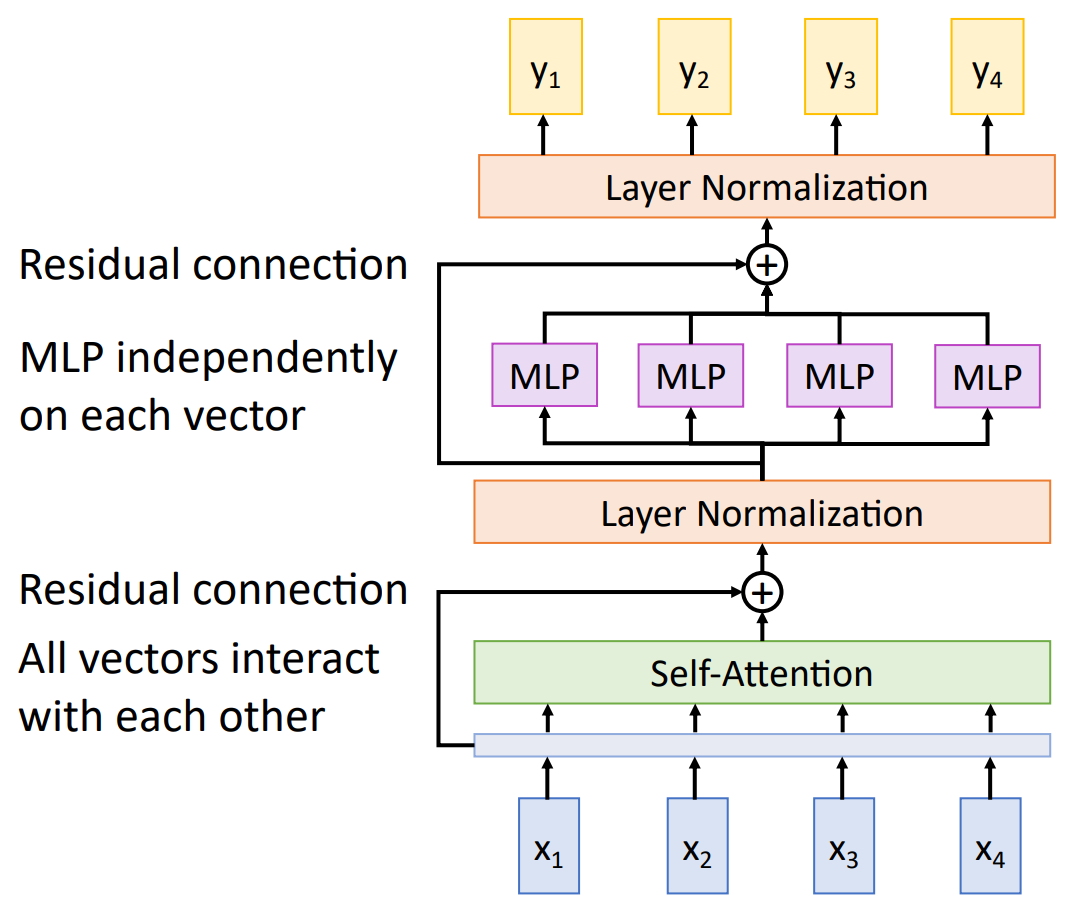
\includegraphics[width=1.0\textwidth,height=0.9\textheight,keepaspectratio]{images/advanced-cv/transformers_2.png}
        \end{figure} 
    \end{column}
\end{columns}

\end{frame}

\begin{frame}{Transformers}

\begin{itemize}
    \item A Transformer consists of a sequence of transformer blocks.
    \item Vaswani et al.\ used 12 blocks, $D_Q = 512$, and 6 attention heads.
\end{itemize}

\begin{figure}
\centering
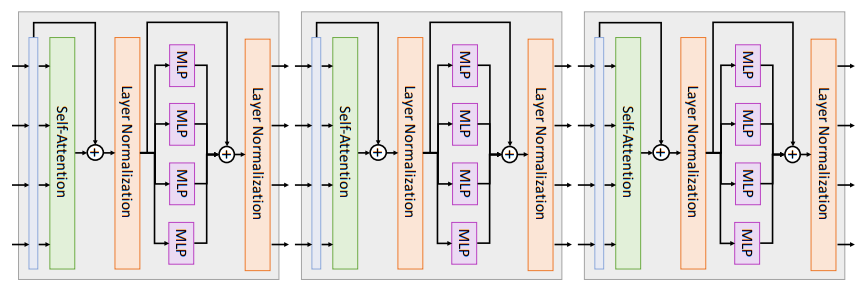
\includegraphics[width=1.0\textwidth,height=1.0\textheight,keepaspectratio]{images/advanced-cv/transformers_3.png}
\end{figure} 
    
\end{frame}
